% Working presentation: internal finite-law IRFs, not full equilibrium validation.
\documentclass[aspectratio=169,11pt]{beamer}
\usepackage[utf8]{inputenc}
\usepackage[T1]{fontenc}
\usepackage[spanish,es-nodecimaldot]{babel}
\usepackage{lmodern,amsmath,amssymb,booktabs,graphicx}
\usetheme{default}
\usecolortheme{seahorse}
\setbeamertemplate{navigation symbols}{}
\setbeamertemplate{footline}[frame number]
\setbeamerfont{frametitle}{size=\large}
\title{Política monetaria, liquidez bancaria\\y asignación de capital}
\subtitle{Entorno NK cerrado y respuestas dinámicas internas}
\author{Alejandro Ventura}
\date{Borrador para revisión: 2 de noviembre de 2026}
\begin{document}
\begin{frame}[plain]\titlepage
\centering\footnotesize
\url{https://github.com/alejandroventuraventurameza-tech/ai-project}
\end{frame}

\begin{frame}{Pregunta y resultado que sometemos a revisión}
¿Cuándo una intervención monetaria facilita capital a empresas productivas?
\medskip
\[
\text{Banco central}\longrightarrow\text{interbancario}\longrightarrow
\text{bancos comerciales}\longrightarrow\text{empresas}.
\]
\begin{itemize}
\item El experimento interno conserva dos ramas del sistema reducido.
\item En ambas baja la tasa de crédito y aumenta el crédito de H.
\item La pérdida asignativa cae en S y sube en B: el signo es condicional.
\end{itemize}
\medskip
\textbf{Alcance:} parámetros ilustrativos, pagos finitos e IRF locales;
la correspondencia completa con equilibrio óptimo sigue pendiente.
\end{frame}

\begin{frame}{Entorno, decisiones y secuencia}
Economía cerrada: hogar trabajador, empresarios H y L, bancos, mercado OTC,
productores de capital, minoristas con ajuste de precios y sector público.
\begin{enumerate}
\item Llegan el estado agregado y las posiciones nominales heredadas.
\item Se produce con capital instalado; se paga trabajo y se liquidan promesas.
\item Empresarios eligen consumo, capital siguiente y financiación.
\item Bancos eligen cartera; llegan pagos idiosincráticos y se liquidan vía OTC/facilidad.
\item Se determina patrimonio futuro, salida y renovación bancaria.
\end{enumerate}
El modelo general incluye incertidumbre agregada. Estas IRF condicionan los
shocks agregados futuros a cero; conservan pagos idiosincráticos binarios.
\end{frame}

\begin{frame}{Empresa: qué maximiza y qué la limita}
\[
V_i(N,\mathcal S)=\max_{c,k',b,a}\{u_E(c)+\beta_E\mathbb E V_i(N',\mathcal S')\}.
\]
\[
c+q_t k'+a=N+b,\qquad
R^L_t b\leq\theta_i(1-\delta)\inf_{s'}\{\Pi_{t+1}q_{t+1}\}\,k'.
\]
\begin{itemize}
\item Caja: consumo, inversión y ahorro se financian con patrimonio y préstamo.
\item Garantía: el repago nominal debe estar cubierto en cada estado admisible.
\item Una tasa menor amplía capacidad financiable a garantía dada, pero precios,
patrimonio y demandas también reaccionan.
\item $A_H>A_L$ no garantiza por sí solo una mejora asignativa.
\end{itemize}
\end{frame}

\begin{frame}{Bancos comerciales y mercado interbancario}
\[
l^B+m^B=d^D+x,\quad x=e-d^B>0,\quad
 d^D\leq\kappa_Dx,\quad l^B\leq\kappa_Lx.
\]
El banco maximiza dividendos y valor futuro descontado, con salida y solvencia
por estado. Después del pago, su exceso de reservas sobre encaje es
\[
s^B=m^B-\rho d^D+(R^D/R^R-\rho)\omega d^D.
\]
\begin{itemize}
\item El interbancario redistribuye reservas entre bancos con déficit y excedente.
\item La facilidad del banco central cubre parte del déficit no negociado.
\item Crédito a empresas y crédito entre bancos son contratos diferentes.
\end{itemize}
Los instrumentos son remuneración y cantidad de reservas, encaje y corredor.
Aquí variamos solo la innovación de remuneración.
\end{frame}

\begin{frame}{Antecedentes y contribución que buscamos}
\begin{itemize}
\item González, Nuño y Thaler, enero de 2026: política monetaria, heterogeneidad
empresarial y mala asignación. Esa relación general ya existe en la literatura.
\item Bianchi y Bigio (2022): reservas, depósitos y gestión de liquidez bancaria.
\item Nuestro candidato conecta implementación monetaria, liquidación,
contrato nominal de colateral y dos respuestas asignativas locales.
\end{itemize}
\medskip
La contribución debe evaluarse con las hipótesis y la revisión de literatura.
El costo cuadrático del laboratorio estático anterior es una simplificación
propia; no se atribuye directamente a Bianchi y Bigio.
\end{frame}

\begin{frame}{Experimento reproducible y significado de las ramas}
\begin{itemize}
\item Innovación $v_{R,0}=-10^{-5}$: aproximadamente $-0.1$ pb en el log de la regla.
\item Mismos estados heredados y anuncios posteriores; comparación con la misma
trayectoria de referencia, no necesariamente estacionaria en el prefijo.
\item S: H restringida, L prestataria con holgura de colateral inicial.
\item B: ambas firmas restringidas inicialmente. No seleccionamos una rama.
\item Pagos $\omega=\pm0.2$, probabilidad $1/2$; trimestre ilustrativo, sin datos reales.
\item Prefijo de dos fechas no lineal; continuación recurrente local lineal.
\end{itemize}
Tasas: diferencias en pb por período, sin anualizar. Cantidades: log \%.
\end{frame}

\begin{frame}{Transmisión financiera: las dos respuestas}
\centering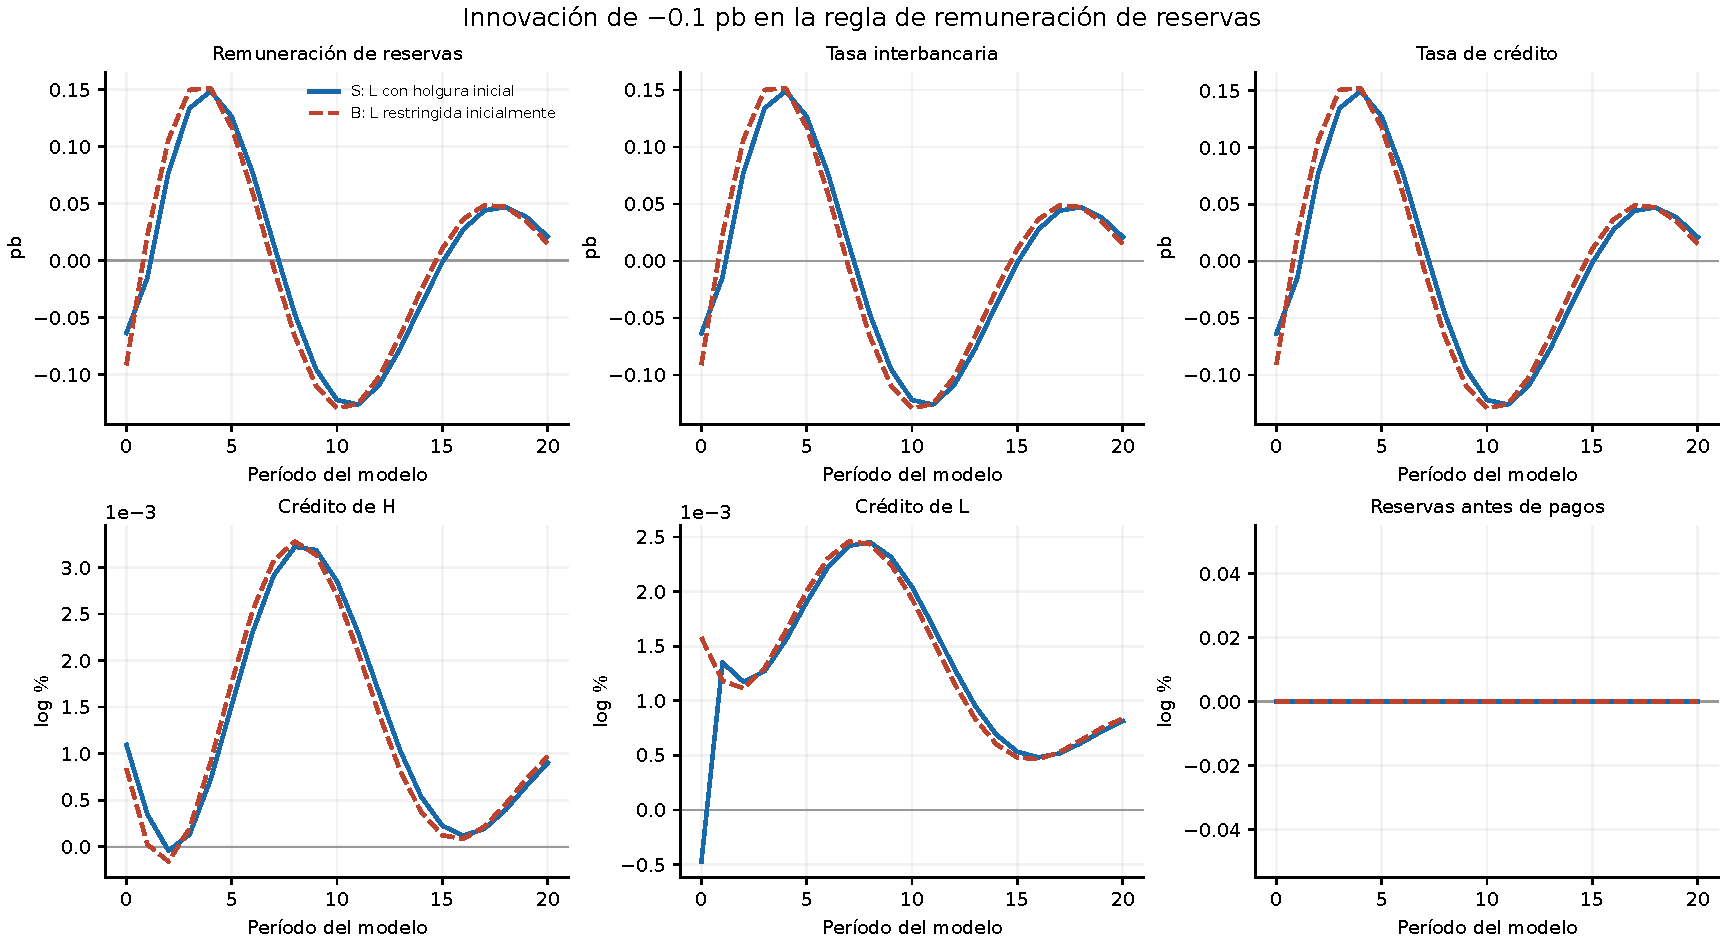
\includegraphics[height=.79\textheight,width=\textwidth,keepaspectratio]{../paper/figures/irf_transmission.pdf}
\end{frame}

\begin{frame}{Capital, producción y pérdida asignativa}
\centering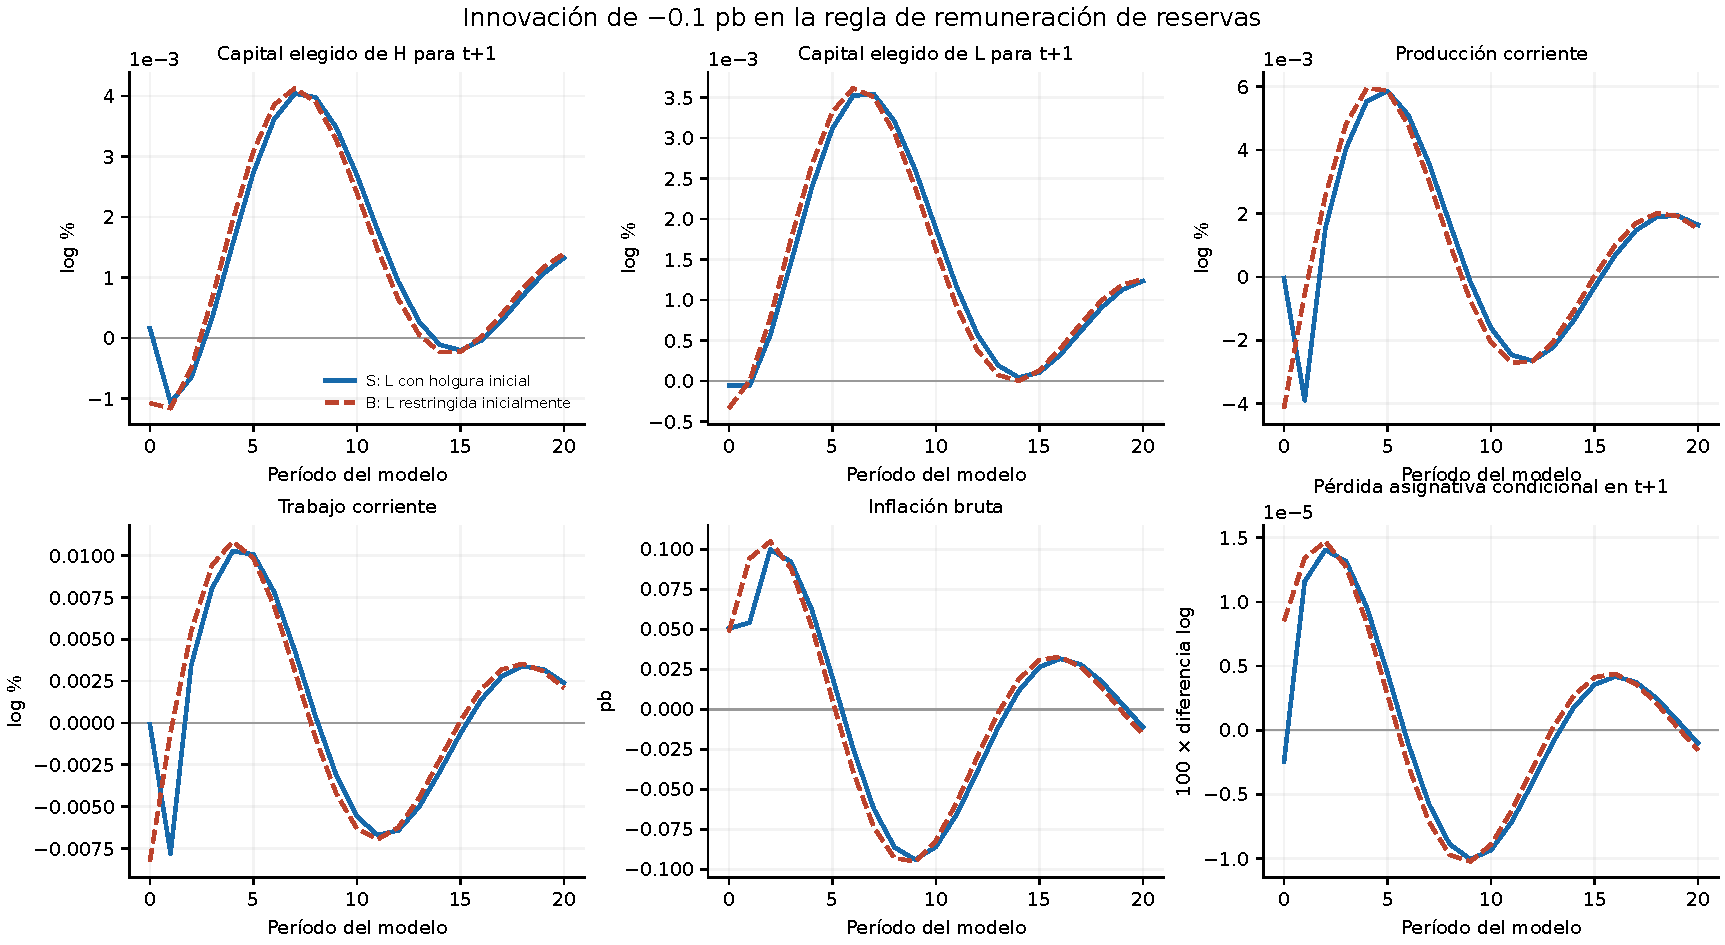
\includegraphics[height=.79\textheight,width=\textwidth,keepaspectratio]{../paper/figures/irf_real_allocation.pdf}
\end{frame}

\begin{frame}{Qué ocurre al impacto}
\centering\small\begin{tabular}{lrr}\toprule
Respuesta al impacto & S & B\\\midrule
Tasa interbancaria (pb) & -0.06363254 & -0.09117145\\
Tasa de crédito (pb) & -0.06363175 & -0.09090760\\
Producción (log \%) & -0.00003580 & -0.00414255\\
Crédito H (log \%) & 0.00109518 & 0.00084065\\
Crédito L (log \%) & -0.00047390 & 0.00157811\\
Pérdida condicional ($100\Delta\log$) & -0.00000248 & 0.00000852\\
\bottomrule\end{tabular}

\medskip\par\raggedright
La pérdida es $\log(Y^{ef}_{t+1}/Y_{t+1})$ a recursos agregados dados del período
siguiente. No mide bienestar ni identifica una fricción financiera con datos.
\end{frame}

\begin{frame}{La producción cae inicialmente: resultado que debemos explicar}
El capital instalado es predeterminado y el trabajo cae en ambos tipos.
Para la tecnología del ejercicio, la condición laboral implica al impacto:
\[
\Delta\log\ell_i=2(\Delta\log m-\Delta\log w),\qquad
\Delta\log y_i=\tfrac12\Delta\log\ell_i.
\]
\[
\Delta Y=\Delta C+\Delta\Gamma+\Delta\mathcal R.
\]
\begin{itemize}
\item El reproductor verifica las identidades laborales y de recursos.
\item Crédito más barato no implica mayor producción corriente automáticamente.
\item Estas identidades ubican el ajuste inmediato; la interpretación estructural
completa requiere cerrar optimalidad y equilibrio. No imponemos el signo.
\end{itemize}
\end{frame}

\begin{frame}{Qué comprobamos y qué no está cerrado}
\begin{itemize}
\item Pasan residuos del prefijo, márgenes de régimen y error de cola del choque pequeño.
\item Tolerancia más estricta y horizonte 320 conservan las respuestas comunes.
\item Choque $-1$ pb: falla el umbral de error de aproximación; no se promueve.
\item Lean: pruebas auxiliares y construcciones condicionales en campaña preliminar.
\item Certificado externo de existencia reducida $\neq$ equilibrio completo probado.
\end{itemize}
\medskip
Pendientes: conectar trayectoria y cotas con todas las hipótesis, aplicar
condiciones terminales, demostrar optimalidad dinámica y correspondencia completa.
\end{frame}

\begin{frame}{Resultado para discusión y siguiente paso}
\textbf{Hallazgo del ejercicio:} la misma innovación puede generar respuestas
asignativas opuestas según la rama, aunque ambas abaraten el crédito.
\medskip
\begin{itemize}
\item Conservar las dos ramas y sus condiciones.
\item Revisar el mecanismo que determina producción y trabajo al impacto.
\item Completar la validación interna antes de estimar o calibrar con datos.
\end{itemize}
\medskip
Reproducción: \texttt{python code/verify.py}.
\par Artículo extenso, tablas automáticas y figuras disponibles para revisión.
\end{frame}
\end{document}
